\documentclass[12pt]{article}

\usepackage[margin=1in,headheight=15pt]{geometry}
\usepackage{amsmath}
\usepackage{amssymb}
\usepackage{graphicx}
\usepackage{float}
\usepackage{hyperref}
\usepackage{booktabs}
\usepackage{caption}
\usepackage{enumitem}
\usepackage{fancyhdr}
\usepackage{setspace}
\usepackage{titlesec}
\usepackage{cite}
\usepackage{listings}
\usepackage{xcolor}

\pagestyle{fancy}
\fancyhf{}
\rhead{ECE 445 --- Individual Progress Report}
\lhead{Prakhar Gupta}
\rfoot{Page \thepage}

\lstset{
  basicstyle=\ttfamily\small,
  keywordstyle=\color{blue},
  commentstyle=\color{gray},
  breaklines=true,
  frame=single,
  language=C
}

\title{
  \textbf{ECE 445 Individual Progress Report} \\
  \large BetaSpray: Automated Climbing Route Projection System \\[0.5em]
  \normalsize Prakhar Gupta (\texttt{prakhar7}), Team 41 \\
  University of Illinois Urbana--Champaign \\
  ECE 445 --- Spring 2026
}
\date{}

\begin{document}

\maketitle
\thispagestyle{fancy}

\setstretch{0.95}

% ===========================================================================
\section{Introduction}
% ===========================================================================

\subsection{Team Project Overview}

BetaSpray is a device that projects laser indicators onto climbing holds on a
``spray wall''---a densely populated wall of random holds found in climbing
gyms.  Existing solutions such as the MoonBoard~\cite{moonboard} require
purpose-built walls with integrated LEDs in regularly spaced holds.  BetaSpray
instead works with \emph{any} existing spray wall: a camera captures the wall,
computer vision detects hold locations, the user selects a route through a web
interface, and servo-actuated laser gimbals highlight the next holds in the
sequence.

The system is built around an ESP32-S3 microcontroller running custom firmware
in C on the ESP-IDF framework.  The three primary subsystems are:

\begin{enumerate}
  \item \textbf{Vision / Camera Subsystem}---An OV5640 camera connected over
        a DVP parallel interface, providing wall images for hold detection.
  \item \textbf{Projection Subsystem}---Four two-axis servo gimbals, each
        carrying a laser module, driven by PWM via the ESP32-S3 LEDC peripheral.
  \item \textbf{User Interface Subsystem}---A Wi-Fi soft-AP HTTP server
        exposing REST endpoints for route management, camera control, and servo
        commands.
\end{enumerate}

\subsection{My Responsibilities and Roles}

Per the team contract, my responsibilities are: (1)~vision subsystem schematic
(camera DVP interface in KiCad), (2)~initial PCB layout (4-layer, later
revised to 2-layer), (3)~the full firmware stack (Wi-Fi, HTTP server, camera
driver, FatFS, route management), (4)~the pixel-to-servo control algorithm,
and (5)~co-designing the 3D-printed enclosure with Max in Fusion~360.

Teammate Ingi Helgason owns the power subsystem schematic, the
Difference-of-Gaussian hold detection algorithm, and extended our Python
client with a REPL shell.  Teammate Max Beach owns the servo power subsystem
PCB, the low-level LEDC servo driver and fade/hold tuning, camera calibration
tooling, and the tiled high-resolution capture mode.  My firmware provides
the HTTP and route-management infrastructure both teammates depend on.

\subsection{Accomplishments, Current Work, and Remaining Tasks}

Completed: the full firmware stack (Wi-Fi, HTTP, FatFS, camera, route
management) running on the devkit; vision subsystem schematic; initial PCB
layout (v0, 4-layer); pixel-to-servo mapping tested at the breadboard demo;
and the first 3D-printed enclosure.

Current work: tuning the coordinate transform for multi-gimbal operation and
integrating Ingi's hold detection output into the route creation workflow.
Remaining: full-system integration on the custom PCB, end-to-end field
testing at a climbing wall, and the final demonstration.


% ===========================================================================
\section{Design}
% ===========================================================================

\subsection{PCB Design---Vision Subsystem Schematic}

I created the vision subsystem schematic sheet in KiCad, defining the
electrical interface between the ESP32-S3 and the OV5640 camera module.  The
OV5640 uses a DVP (Digital Video Port) parallel interface for image data
transfer.  Our purchased camera module comes on a breakout board, so the first
PCB revision uses two 9-pin connectors to interface with it.

The DVP pin mapping is summarized in Table~\ref{tab:dvp_pins}.

\begin{table}[H]
  \centering
  \caption{OV5640 DVP pin mapping to ESP32-S3.}
  \label{tab:dvp_pins}
  \begin{tabular}{llp{7cm}}
    \toprule
    Signal & Direction & Description \\
    \midrule
    D2--D9 & Input & 8-bit parallel pixel data bus \\
    HREF   & Input & Horizontal reference (line valid) \\
    VSYNC  & Input & Vertical sync (frame valid) \\
    PCLK   & Input & Pixel clock \\
    SDA/SCL & Bidir/Input & I\textsuperscript{2}C (SCCB) for camera config \\
    PWDN   & Output & Power-down (active high) \\
    RESET  & Output & Reset (active low) \\
    \bottomrule
  \end{tabular}
\end{table}

A critical constraint was avoiding the ESP32-S3's reserved pins.  I
documented exclusion zones on the schematic~\cite{espidf}: strapping pins
(GPIO0/3/45/46), PSRAM SPI (GPIO35--37), UART (GPIO43/44), USB (GPIO19/20),
and JTAG (GPIO39--42).  XCLK was left unconnected (we use the OV5640's
internal 24\,MHz oscillator~\cite{adafruit_ov5640}).  I also added laser
module connections (2N2222 BJT switch from GPIO, 5\,V rail), servo signal
labels, and a debug LED.

\subsection{PCB Layout---Initial 4-Layer Board (v0)}

I performed the initial PCB layout on a 99.4\,mm~$\times$~99.4\,mm board
with a 4-layer stackup: component placement, DVP/I\textsuperscript{2}C/PWM
signal routing, ground and power plane stitching, and mounting holes per
machine shop specs.  The 4-layer stackup provided clean power/ground planes,
but after reviewing PCBWay pricing (significantly higher for 4-layer) and
the fact that our signal frequencies (24\,MHz PCLK, 50\,Hz PWM) do not
strictly require inner planes, the team moved to a 2-layer board.  Ingi led
the 2-layer revision, carrying forward my v0 placement and routing.

During assembly I discovered a footprint error: the camera connector was
3.96\,mm pitch instead of 2.54\,mm.  I fixed the footprint immediately and
the team ordered replacement ribbon cables to continue testing other
subsystems while a corrected board was submitted.

\begin{figure}[H]
  \centering
  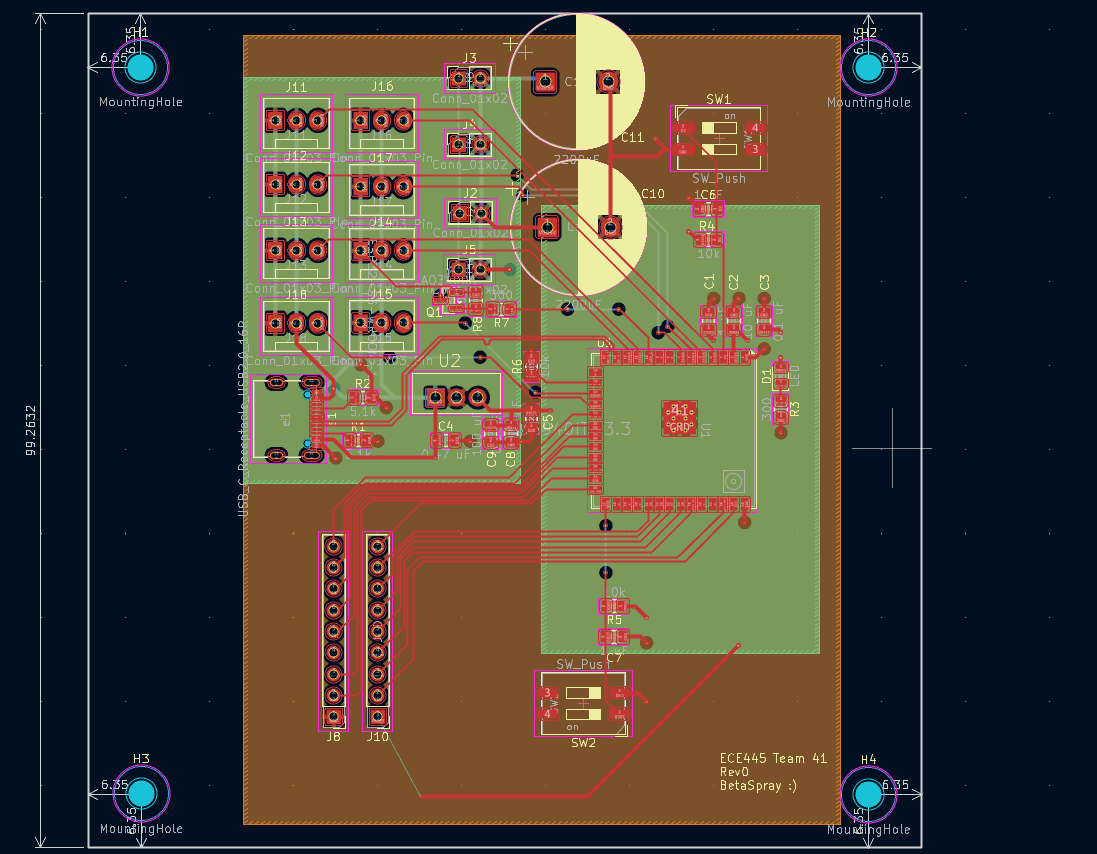
\includegraphics[width=0.7\textwidth]{img/pcb.png}
  \caption{KiCad PCB layout showing component placement and routing.}
  \label{fig:pcb_layout}
\end{figure}

\subsection{Firmware Architecture}

The embedded firmware is structured as a set of loosely coupled modules, each
with its own \texttt{.c}/\texttt{.h} pair.  I authored all of the following
modules: \texttt{wifi.c}, \texttt{server.c}, \texttt{camera.c},
\texttt{fatfs.c}, and \texttt{route.c}, as well as the initialization
sequence in \texttt{main.c}.  The servo driver (\texttt{servo.c}) was
initially written by me and later extended by Max with fade/hold tuning logic.

\subsubsection{Wi-Fi Soft Access Point}

The \texttt{wifi.c} module configures the ESP32-S3 as a Wi-Fi soft access
point (SSID: \texttt{BetaSpray}, WPA2).  We chose soft AP over station mode
(connecting to an existing router) to eliminate dependence on gym
infrastructure---the device works anywhere without credentials or network
access.  A wired serial fallback was considered in the proposal but proved
unnecessary once soft AP demonstrated reliable short-range performance.

During bringup, the board crashed on boot with
\texttt{ESP\_ERR\_INVALID\_STATE} inside
\texttt{esp\_netif\_create\_default\_wifi\_ap()}.  The root cause was that
\texttt{esp\_event\_loop\_create\_default()} must be called before any Wi-Fi
initialization---an ordering dependency that the ESP-IDF documentation does
not make explicit~\cite{espidf}.  The fix was to ensure the default event loop
and NVS flash are both initialized at the top of \texttt{app\_main} before
any peripheral bringup.

\subsubsection{HTTP Server}

The \texttt{server.c} module implements a REST API with 15 endpoints using
the ESP-IDF \texttt{httpd} library.  The endpoints fall into four functional
groups, summarized in Table~\ref{tab:endpoints}.

\begin{table}[H]
  \centering
  \caption{HTTP server REST API endpoints.}
  \label{tab:endpoints}
  \begin{tabular}{lll}
    \toprule
    Endpoint & Method & Function \\
    \midrule
    \texttt{/capture}        & POST & Trigger camera capture \\
    \texttt{/get}            & GET  & Retrieve stored JPEG frame \\
    \texttt{/configure}      & POST & Camera settings (enable/disable, format) \\
    \texttt{/servo}          & POST & Command individual servo \\
    \texttt{/route/create}   & POST & Create route from JSON hold array \\
    \texttt{/route/delete}   & POST & Delete route file from flash \\
    \texttt{/route/load}     & POST & Load route from flash into RAM \\
    \texttt{/route/play}     & POST & Load and begin route playback \\
    \texttt{/route/pause}    & GET  & Pause playback \\
    \texttt{/route/next}     & GET  & Advance to next hold \\
    \texttt{/route/restart}  & POST & Restart route from beginning \\
    \texttt{/route/mapping}  & POST & Set pixel-to-angle transform params \\
    \texttt{/start}          & GET  & Begin projection \\
    \texttt{/stop}           & GET  & Stop projection \\
    \texttt{/test}           & POST & Echo test \\
    \bottomrule
  \end{tabular}
\end{table}

All POST endpoints parse JSON request bodies using the cJSON library.
The camera capture path stores the most recent frame in a static DRAM buffer
(PSRAM allocation is planned for the custom PCB with the ESP32-S3FH4R2
module, which has 8\,MB of PSRAM).

An early bug was that the capture handler allocated the frame buffer on the
stack inside the HTTP handler, which caused stack overflows when the handler
was invoked from the \texttt{httpd} task (which has a limited stack).  Moving
to a static buffer with \texttt{malloc} (and later \texttt{heap\_caps\_malloc}
for PSRAM-aware allocation) resolved this.

\subsubsection{FatFS Flash Storage}

I proposed using the ESP32-S3 WROOM module's integrated SPI flash for
persistent route storage rather than adding an external SD card---the
internal flash requires no additional hardware, and ESP-IDF provides a
mature FatFS integration with wear-levelling.  The \texttt{fatfs.c} module
implements this filesystem layer.  A custom
\texttt{partitions.csv} was required since the default partition table does
not include a FAT partition:

\begin{table}[H]
  \centering
  \caption{Custom flash partition table.}
  \label{tab:partitions}
  \begin{tabular}{lll}
    \toprule
    Partition & Offset & Size \\
    \midrule
    nvs           & \texttt{0x9000}   & 24\,KB \\
    phy\_init     & \texttt{0xF000}   & 4\,KB \\
    factory       & \texttt{0x10000}  & 1\,MB \\
    storage (FAT) & \texttt{0x110000} & 960\,KB \\
    \bottomrule
  \end{tabular}
\end{table}

The module exposes create, read, write, delete, and list operations.  Read
and write accept an offset and size parameter for chunked access without
loading entire files into DRAM.

\subsubsection{Camera Driver Integration}

The \texttt{camera.c} module wraps the Espressif \texttt{esp32-camera}
component, configuring the OV5640 for QVGA (320$\times$240) JPEG capture
over the DVP parallel interface.  We originally planned to run hold detection
entirely on the ESP32-S3, but early testing showed that even downsampled
images took several seconds to process on-device.  We shifted the CV pipeline
to a host PC, freeing the ESP32-S3 for HTTP serving, route management, and
servo control.  The initial PCB uses the WROOM-1U module (integrated crystal,
flash, antenna matching); the final revision targets the bare ESP32-S3FH4R2
with wirebonded 8\,MB PSRAM for full-resolution captures.  Key configuration
decisions:

\begin{itemize}
  \item \textbf{Frame buffer location}: \texttt{CAMERA\_FB\_IN\_DRAM} on the
        N8 devkit (no PSRAM); the custom PCB uses the ESP32-S3FH4R2 (N16R8)
        with 8\,MB PSRAM for higher-resolution captures.
  \item \textbf{Single frame buffer} (\texttt{fb\_count = 1}) to conserve
        memory.
  \item \textbf{LEDC timer isolation}: the camera's XCLK generator uses
        \texttt{LEDC\_TIMER\_1} / \texttt{LEDC\_CHANNEL\_7}, while the servo
        driver uses \texttt{LEDC\_TIMER\_0} / channels~0--7.  This prevents
        timer conflicts when both subsystems operate simultaneously.
  \item \textbf{JPEG quality~12} (scale 0--63, lower is better) as a balance
        between image quality and buffer size at QVGA resolution.
\end{itemize}

During bringup, an attempt to allocate the frame buffer from PSRAM failed
silently on the N8 devkit (which lacks PSRAM).  Ingi identified this during
testing; switching to DRAM allocation resolved the issue.

\begin{figure}[H]
  \centering
  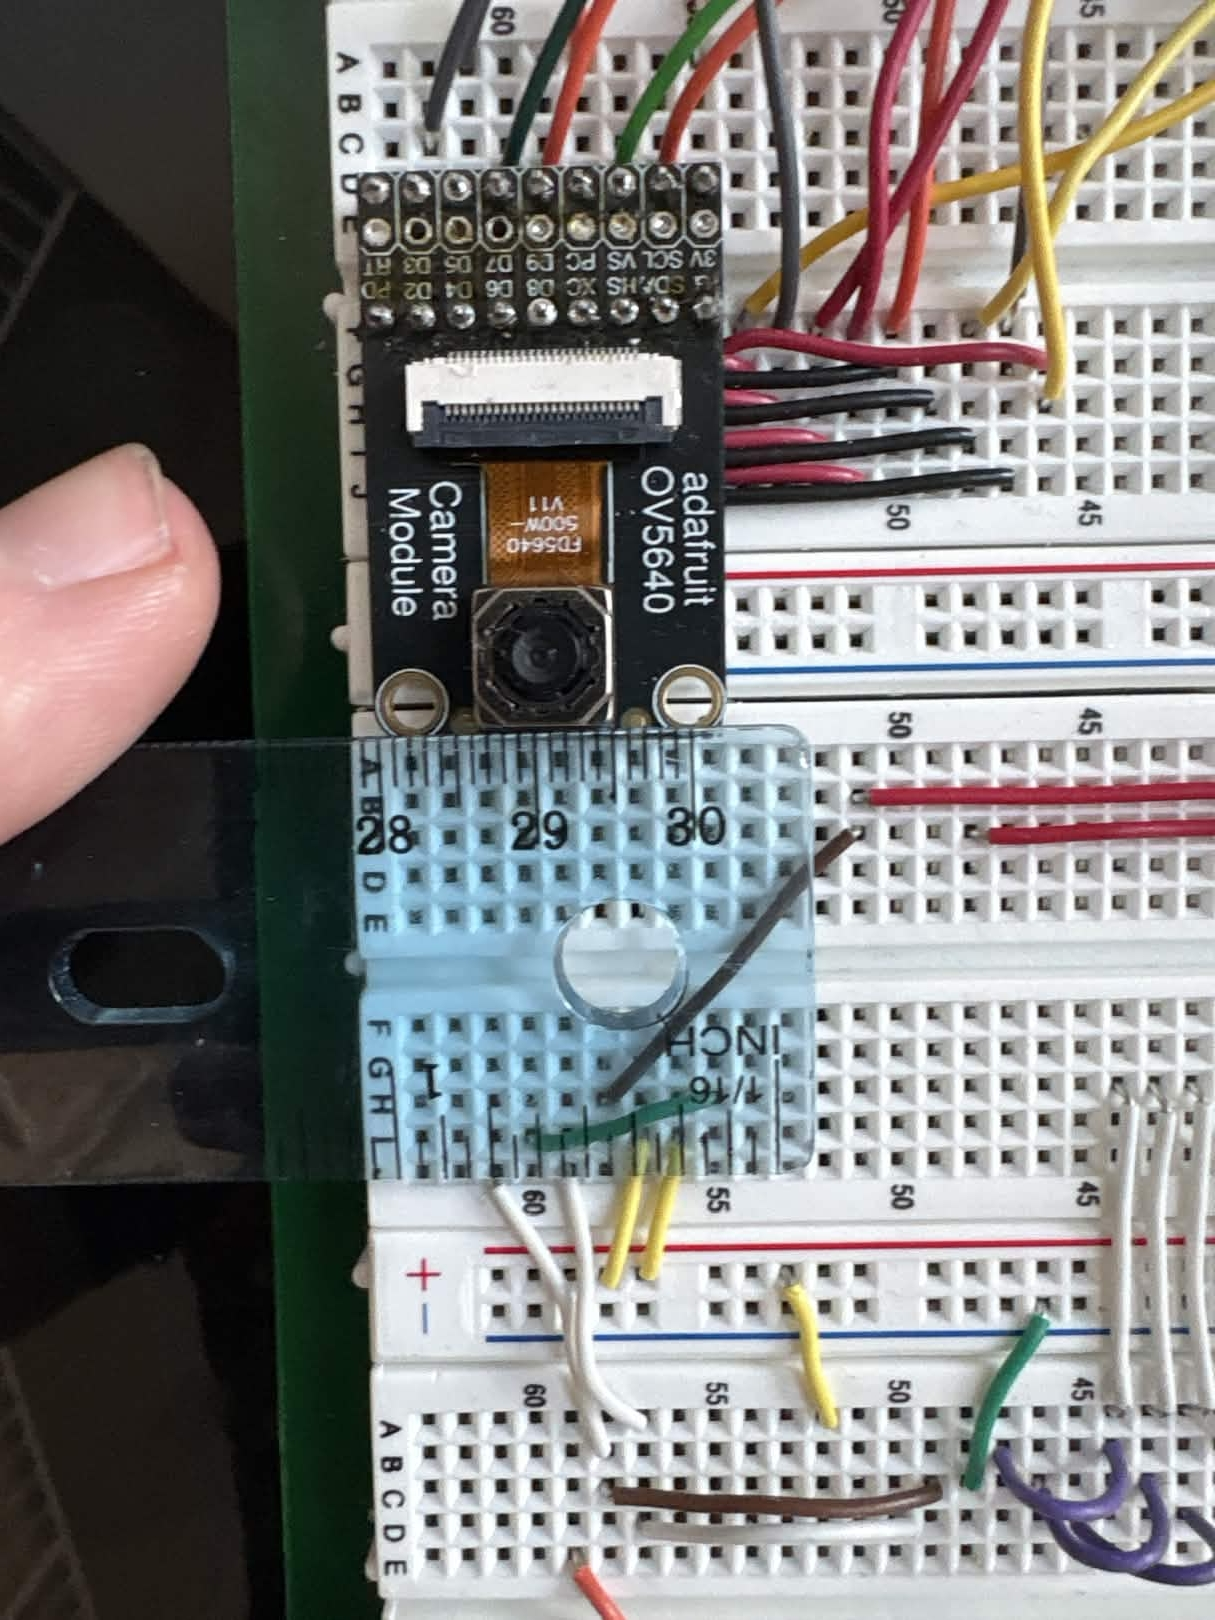
\includegraphics[width=0.5\textwidth]{img/example-wiring.jpg}
  \caption{OV5640 camera module wired to the ESP32-S3 devkit breadboard
  via DVP parallel interface for the demo.}
  \label{fig:wiring}
\end{figure}

\subsubsection{Route Management System}

The \texttt{route.c} module is the core of the projection pipeline, bridging
hold detection output to servo actuation.  It provides:

\begin{enumerate}
  \item \textbf{Route CRUD}: routes are stored as binary files on FatFS at
        \texttt{/fatfs/routeN.xy}.  We debated storing servo angles directly,
        but this would couple route data to a specific device placement---if
        the device moves, all saved routes break.  Instead, the binary format
        stores camera-space pixel coordinates (4-byte hold count followed by
        interleaved \texttt{float32} $x, y$ pairs, max 516~bytes for 64
        holds), and the angular conversion is computed at playback time via
        the runtime-configurable transform.  This also avoids JSON parsing
        overhead on the microcontroller.

  \item \textbf{Playback task}: a dedicated FreeRTOS task
        (\texttt{route\_playback\_task}) runs at priority~5 and iterates
        through the loaded holds.  For each hold, it computes servo angles via
        the pixel-to-servo transform (Section~\ref{sec:control}), drives the
        appropriate gimbal, and waits for either a configurable dwell timeout
        (auto-advance mode, 3\,s default) or a manual \texttt{/route/next}
        command.  Synchronization uses a binary semaphore for the next-hold
        signal and a mutex for shared state (current hold index, playing flag).

  \item \textbf{Runtime-configurable transform}: the \texttt{/route/mapping}
        endpoint accepts camera FOV (horizontal and vertical, in degrees),
        image dimensions (pixels), and wall distance (meters), allowing the
        coordinate transform to be reconfigured without reflashing.
\end{enumerate}

\subsection{Pixel-to-Servo Control Algorithm}
\label{sec:control}

Converting camera-space pixel coordinates to servo angles bridges the vision
and projection subsystems.  The transform assumes the camera is co-located
with the gimbal assembly and the wall is approximately planar at distance~$d$.

For the horizontal (X) axis, a pixel at position $p_x$ in an image of width
$W$ with horizontal field of view $\theta_H$ maps to a servo angle:

\begin{equation}
  \alpha_x = \left(\frac{p_x - W/2}{W}\right) \cdot \theta_H + 90^\circ
  \label{eq:servo_x}
\end{equation}

\noindent where 90\textdegree{} is the servo center position.  The term
$(p_x - W/2)/W$ normalizes the pixel offset from center to the range
$[-0.5, +0.5]$, which is then scaled by the field of view.

For the vertical (Y) axis, the convention is inverted (pixel $y = 0$ is the
top of the image, but the servo's 90\textdegree{} corresponds to horizontal):

\begin{equation}
  \alpha_y = 90^\circ + \left(\frac{H - p_y}{H}\right) \cdot \theta_V
  \label{eq:servo_y}
\end{equation}

\noindent where $H$ is the image height and $\theta_V$ is the vertical field
of view.  Both outputs are clamped to $[0^\circ, 180^\circ]$ to stay within the SG90's
mechanical range.

Two issues arose during testing: (1)~large angular jumps caused overshoot,
which Max mitigated with LEDC fade/hold tuning while I added FOV/2 clamping
to keep servos within the camera's visible range; (2)~the Y-axis mapping was
initially inverted, corrected by the $(H - p_y)$ term in
Equation~\ref{eq:servo_y}.

\begin{figure}[H]
  \centering
  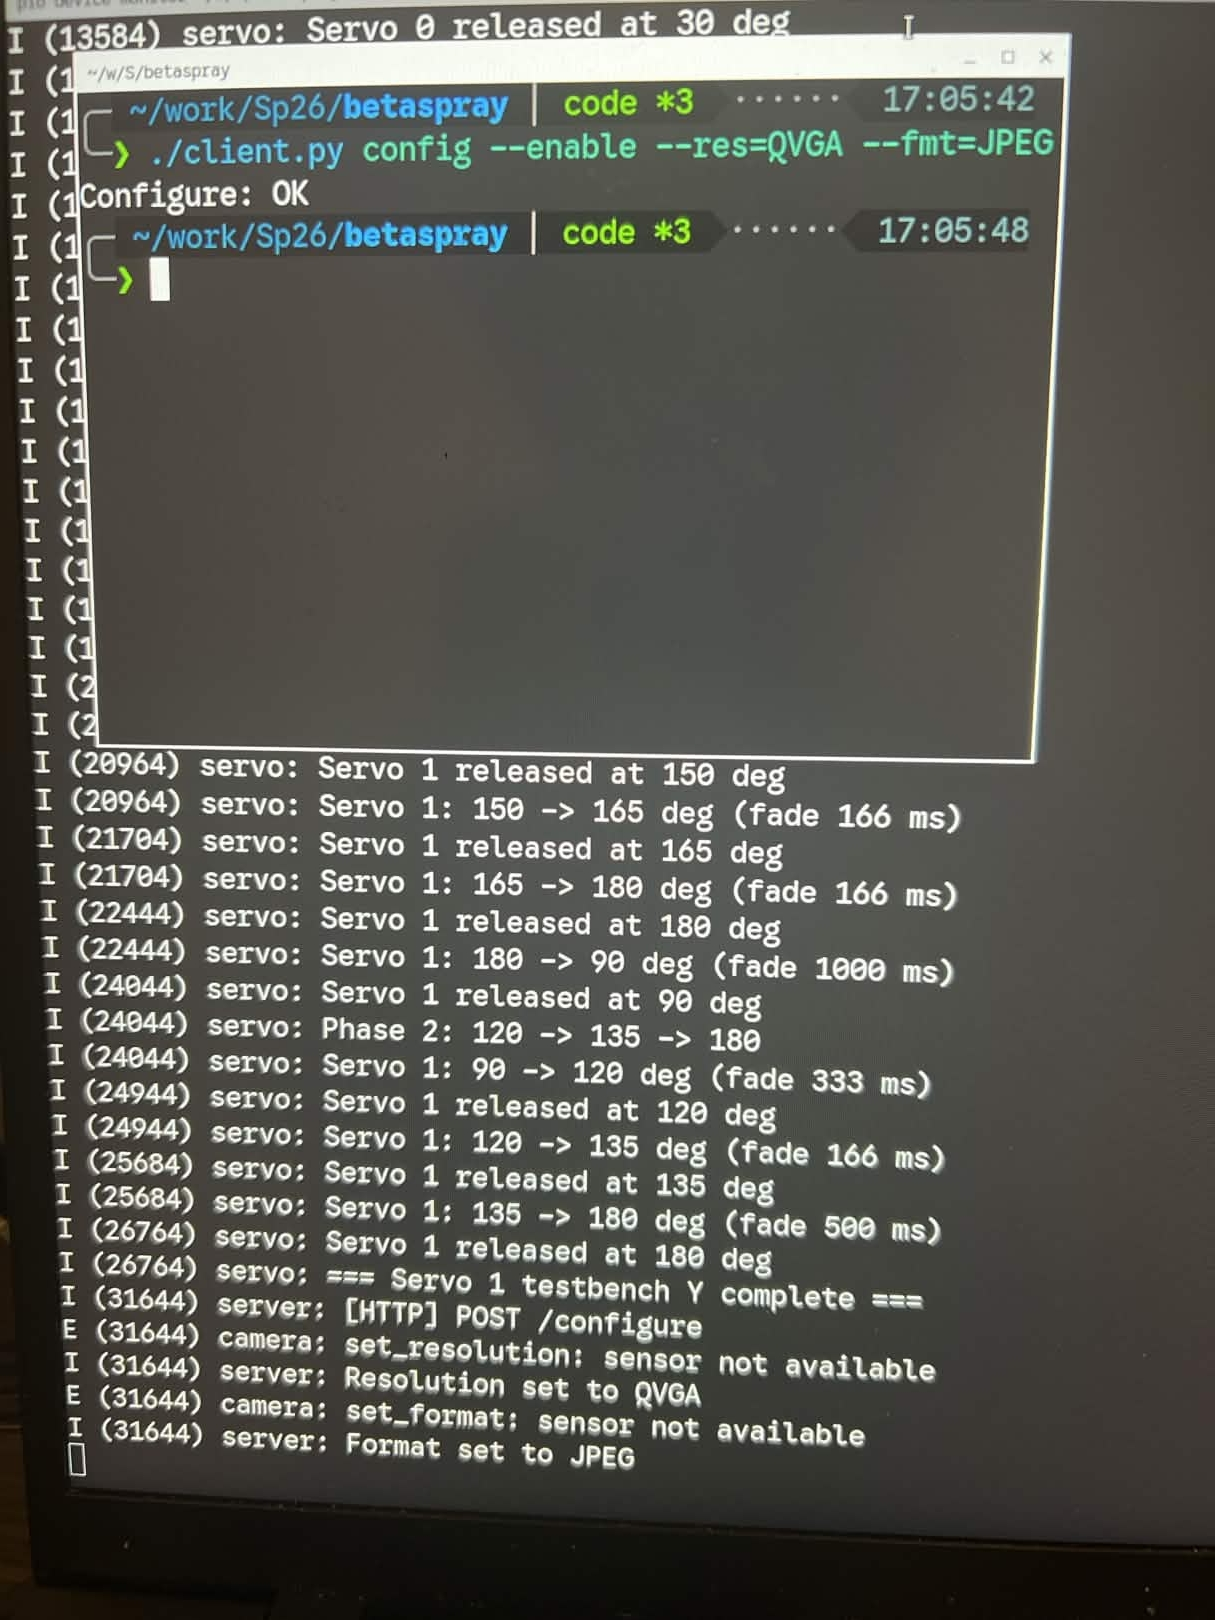
\includegraphics[width=0.7\textwidth]{img/client_config.jpg}
  \caption{Terminal session showing servo testbench output (top) and
  \texttt{client.py} camera configuration commands (bottom).}
  \label{fig:client_terminal}
\end{figure}

\subsection{3D-Printed Enclosure}

I designed the 3D-printed enclosure in Fusion~360, driven by the need to
iterate rapidly on camera placement and gimbal mounting geometry.  The
enclosure accommodates the PCB (with standoffs), four servo gimbals at
staggered heights for laser clearance, and a protruding camera mount.  Max
provided camera mounting hole measurements (1.8\,cm center-to-center, 3\,mm
holes) and submitted the STL to the X1~Carbon print queue ($\sim$4~hour
print time).

\begin{figure}[H]
  \centering
  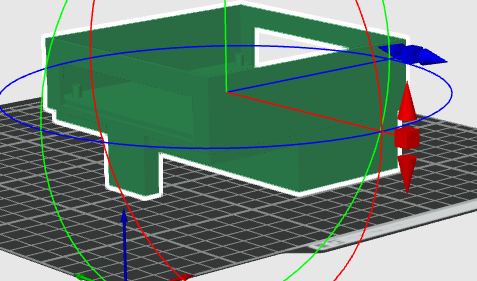
\includegraphics[width=0.7\textwidth]{img/cad.png}
  \caption{Fusion~360 CAD model of the BetaSpray enclosure, showing PCB bay,
  camera mount (right), and gimbal mounting regions.}
  \label{fig:enclosure_cad}
\end{figure}


% ===========================================================================
\section{Verification}
% ===========================================================================

\subsection{Wi-Fi and HTTP Server Verification}

The Wi-Fi soft AP and HTTP server were verified incrementally during bringup.
The first functional test used the \texttt{/test} echo endpoint: a POST
request with an arbitrary string body returns \texttt{ECHO: <body>},
confirming that the TCP/IP stack, HTTP request parsing, and response path are
functional end-to-end.

Subsequent testing used \texttt{client.py}, a Python HTTP client I wrote
(later extended by Ingi with a REPL shell).  On March~7, Ingi and I
debugged the camera path remotely---he tested on hardware while I pushed
fixes, identifying the SPIRAM and stack overflow bugs.

\subsection{FatFS Route Persistence Verification}

Route persistence was tested by creating a route via
\texttt{POST /route/create}, power-cycling the ESP32-S3, then loading the
same route via \texttt{POST /route/load} and verifying that the hold
coordinates in the serial log matched the original values.  The binary file
format was validated by reading the raw bytes via \texttt{fatfs\_read} with
offset~0 and comparing against the expected
\texttt{[uint32 count][float32 x, y]...} layout.

\subsection{Camera Integration Verification}

Camera functionality was verified by:
\begin{enumerate}
  \item Enabling the camera via
        \texttt{POST /configure \{``enabled'': true\}}.
  \item Triggering a capture via \texttt{POST /capture}.
  \item Retrieving the JPEG via \texttt{GET /get} and saving to disk.
  \item Visually inspecting the image for correct framing and exposure.
\end{enumerate}

The LEDC timer isolation between the camera (Timer~1) and servo (Timer~0)
subsystems was confirmed by simultaneously running servo commands and camera
captures without mutual interference or DMA corruption.

\begin{figure}[H]
  \centering
  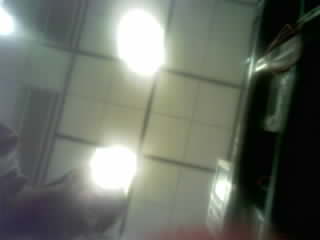
\includegraphics[width=0.5\textwidth]{img/first_image_ever.png}
  \caption{First image captured from the OV5640 over HTTP, taken after
  resolving the DRAM frame buffer allocation failure on the devkit.}
  \label{fig:first_capture}
\end{figure}

\subsection{Route Playback and Servo Mapping Verification}

End-to-end route playback was tested on the breadboard prototype during the
March~8--9 demo preparation sessions:

\begin{enumerate}
  \item The transform parameters were set via \texttt{POST /route/mapping}
        with known FOV values and a wall distance of 3\,m.
  \item A test route was created with holds at known pixel coordinates
        (corners and center of a 320$\times$240 frame).
  \item The route was played back and the laser dot positions were observed
        on a blank wall.
  \item The offset between the laser dot and expected position was estimated
        visually.
\end{enumerate}

During these tests, Ingi performed homing-vs-no-homing repeatability
measurements (approximately 12~iterations per configuration) and found that
dead-reckoning accuracy was sufficient for point-to-point movements exceeding
2--3\textdegree{}, with accumulated error clusters measuring less than
one-half inch in diameter at 3\,m.  This result, combined with Max's servo
repeatability data ($<$1\,cm error at 3\,m), gives confidence that the system
meets the $\pm$5\,cm accuracy requirement at the wall surface.

The FOV/2 clamping fix was validated by commanding holds at extreme pixel
positions ($p_x = 0$ and $p_x = 319$) and confirming the servo did not
exceed the camera's visible angular range.

\begin{figure}[H]
  \centering
  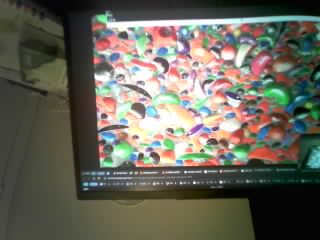
\includegraphics[width=0.7\textwidth]{img/sample_holds.jpg}
  \caption{Climbing wall image displayed on laptop, used as input to the
  hold detection pipeline for route creation testing.}
  \label{fig:holds_input}
\end{figure}

\begin{figure}[H]
  \centering
  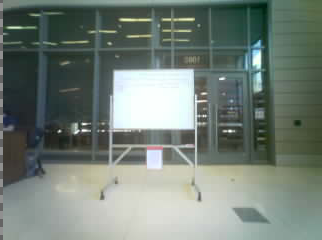
\includegraphics[width=0.7\textwidth]{img/sample_res.png}
  \caption{Whiteboard used to test the pixel-to-servo angular mapping:
  the laser was directed at known pixel coordinates and the resulting
  dot positions were measured to validate the FOV-based conversion.}
  \label{fig:fov_test}
\end{figure}

\subsection{Remaining Verification}

The following tests are planned but not yet complete:

\begin{itemize}
  \item \textbf{Custom PCB integration}: validate the full firmware stack on
        the PSRAM-equipped ESP32-S3FH4R2, particularly camera capture at
        resolutions above QVGA.
  \item \textbf{Multi-gimbal playback}: the breadboard test uses a single
        gimbal (2~servos); full 4-gimbal (8~servo) playback is untested.
  \item \textbf{End-to-end with hold detection}: feed Ingi's DoG output into
        \texttt{/route/create} and verify that projected lasers land on the
        correct physical holds.
  \item \textbf{Climbing wall field test}: project a real route in a gym
        environment under variable lighting and wall angles.
\end{itemize}


% ===========================================================================
\section{Conclusion}
% ===========================================================================

\subsection{Summary}

My contributions span PCB design (vision schematic, v0 4-layer layout,
footprint correction), the full firmware stack (Wi-Fi, HTTP server, FatFS,
camera driver, route management with FreeRTOS playback), the pixel-to-servo
control algorithm ($<$1\,cm error at 3\,m), and a co-designed 3D-printed
enclosure.

\subsection{Timeline and Remaining Work}

\begin{table}[H]
  \centering
  \caption{Remaining milestones.}
  \label{tab:timeline}
  \begin{tabular}{lll}
    \toprule
    Task & Target Date & Status \\
    \midrule
    Custom PCB firmware validation      & April 2026 & Planned \\
    Multi-gimbal playback testing       & April 2026 & Planned \\
    Hold detection $\to$ route integration & April 2026 & In Progress \\
    End-to-end climbing wall demo       & May 2026   & Planned \\
    Final report                        & May 2026   & Planned \\
    \bottomrule
  \end{tabular}
\end{table}

We are roughly on track relative to the design document schedule.
Assembling the corrected PCB and completing subsystem verification is the
top priority for the coming weeks.

\subsection{Self-Assessment}

I could have done a better job with the PCB design review process.  The
camera connector footprint mistake (3.96\,mm pitch instead of 2.54\,mm) was
a straightforward error that should have been caught during schematic review
or by cross-referencing the physical part before submission.  This cost
the team approximately one week of integration time and required ordering
replacement ribbon cables.  Going forward, I will verify every footprint
against the physical component before submitting a board for fabrication.

I also should have pushed for more frequent hardware-in-the-loop testing.
Much of the firmware was written without the board in hand, so bugs like the
SPIRAM allocation issue were not caught until demo prep.  More regular
integration testing would have reduced last-minute pressure.

On the positive side, the modular firmware architecture paid off well.  The
clean separation between \texttt{wifi.c}, \texttt{server.c}, \texttt{camera.c},
\texttt{fatfs.c}, and \texttt{route.c} made it straightforward for Ingi to
extend the client and for Max to add servo tuning without stepping on each
other's code.  The decision to use FatFS for persistent route storage (which
I proposed early in the design phase) also proved valuable, as it enabled
the route-create-power-cycle-reload workflow that is central to the user
experience.

\subsection{Ethical Considerations}

Per the IEEE Code of Ethics~\cite{ieee_ethics}, BetaSpray's primary safety
concern is the use of Class~II laser modules directed at a climbing wall.
We mitigate this with software servo-range limits (FOV/2 clamp), a
\texttt{/stop} endpoint for immediate PWM shutoff, and physical placement
2--3\,m from the wall with beams directed away from eye level~\cite{laser_safety}.
The system transmits only hold coordinates and JPEG frames over a local
Wi-Fi network with no cloud connection, minimizing privacy concerns.

% ===========================================================================
\begin{thebibliography}{9}

\bibitem{moonboard}
Moon Climbing, ``MoonBoard,'' moonboard.com. Accessed: Feb.~12, 2026.

\bibitem{ifsc}
International Federation of Sport Climbing, ``IFSC Rules 2024,''
ifsc-climbing.org. Accessed: Feb.~12, 2026.

\bibitem{laser_safety}
Weill Cornell Medicine, ``Laser Classification,''
https://mhp.weill.cornell.edu/laser-safety/laser-classification.
Accessed: Mar.~30, 2026.

\bibitem{ieee_ethics}
IEEE, ``IEEE Code of Ethics,'' ieee.org/about/corporate/governance/p7-8.html.
Accessed: Mar.~30, 2026.

\bibitem{ov5640}
OmniVision Technologies, ``OV5640 5-Megapixel CMOS Image Sensor,''
Application Note, 2013.

\bibitem{espidf}
Espressif Systems, ``ESP-IDF Programming Guide,'' v5.x,
https://docs.espressif.com/projects/esp-idf/en/latest/.

\bibitem{sg90}
TowerPro, ``SG90 9g Micro Servo,'' Datasheet, 2010.

\bibitem{lm3940}
Texas Instruments, ``LM3940 1-A Low-Dropout Regulator for 5-V to 3.3-V
Conversion,'' SNVS034E, 2013.

\bibitem{adafruit_ov5640}
Instructables, ``ESP32 Webcam with Autofocus Using Adafruit OV5640,''
instructables.com. Accessed: Feb.~24, 2026.

\end{thebibliography}

\end{document}
